% =====================================================================
%  Capítulo 20. Aprendizaje automático en finanzas
% =====================================================================
\chapter[Aprendizaje automático]{Aprendizaje automático en finanzas: contracción, validación y árboles}\label{cap:aprendizaje}

\section*{Objetivos de aprendizaje}
Al terminar este capítulo, el lector podrá:
\begin{enumerate}[label=\arabic*.,leftmargin=*]
  \item Explicar el dilema entre sesgo y varianza y por qué un modelo que ajusta mejor dentro de la muestra puede
        pronosticar peor fuera de ella.
  \item Estimar ridge, lasso y red elástica, derivar sus soluciones y elegir la penalización con validación que
        respete el orden del tiempo.
  \item Evaluar pronósticos de rendimientos fuera de muestra con el $R^2$ fuera de muestra, la prueba de Clark y
        West y su valor económico para un inversionista.
  \item Clasificar eventos con regresión logística y medir la calidad de la clasificación con la curva ROC, y
        reconocer el sobreajuste de los árboles de regresión.
\end{enumerate}

\section*{Motivación}
El aprendizaje automático promete extraer señales de muchas variables con métodos flexibles. En finanzas esa promesa
choca con un hecho del Capítulo~\ref{cap:eficiencia}: los rendimientos son casi impredecibles, de modo que la señal es
diminuta frente al ruido. En ese ambiente, la flexibilidad es peligrosa: un modelo con muchos parámetros ajusta el
ruido de la muestra y pronostica peor que la media histórica. Goyal y Welch (2008) mostraron que casi ningún predictor
clásico de la prima de mercado supera a la media fuera de muestra. Las técnicas de este capítulo, la contracción, la
validación temporal y la combinación de pronósticos, son las herramientas para no engañarse. Gu, Kelly y Xiu (2020)
encontraron ganancias reales con redes y árboles en el corte transversal de miles de acciones; aquí trabajamos con un
problema más pequeño que permite ver cada paso.

\paragraph{Datos del capítulo.} Diez predictores mensuales del exceso de rendimiento del mercado de EE.\,UU. del mes
siguiente, de septiembre de 1927 a noviembre de 2018 ($n=1\,095$), construidos con la base de Robert Shiller y la de
Kenneth French: razón dividendo/precio ($dp$), beneficio/precio ($ep$), dividendo/beneficio ($de$), CAPE, rendimiento del
bono a 10 años ($lty$), tasa de las letras ($tbl$), pendiente ($tms=lty-tbl$), inflación de 12 meses rezagada, momentum de 12
meses y volatilidad de 12 meses del mercado. Para la clasificación, la curva de rendimientos de McCulloch y Kwon del
Capítulo~\ref{cap:tasas} y las recesiones del NBER.

% ---------------------------------------------------------------------
\section{Sesgo, varianza y validación}
% ---------------------------------------------------------------------

Sea $y=f(\mathbf x)+\varepsilon$ con $\E[\varepsilon\mid\mathbf x]=0$ y $\Var(\varepsilon)=\sigma^2$, y sea $\hat f$ un estimador obtenido con una
muestra de entrenamiento independiente de un punto nuevo $(\mathbf x_0,y_0)$.

\begin{proposicion}[Descomposición sesgo-varianza]\label{prop:sesgovarianza}
\[
  \E\bigl[(y_0-\hat f(\mathbf x_0))^2\bigr]=\sigma^2+\bigl[\E\hat f(\mathbf x_0)-f(\mathbf x_0)\bigr]^2+\Var\bigl(\hat f(\mathbf x_0)\bigr).
\]
\end{proposicion}

\begin{proof}
Escribimos $y_0-\hat f=\varepsilon_0+(f-\E\hat f)+(\E\hat f-\hat f)$, donde todo se evalúa en $\mathbf x_0$. El primer término es
independiente de los otros dos (viene del punto nuevo) y el tercero tiene media cero:
\begin{align*}
  \E[(y_0-\hat f)^2] &= \E[\varepsilon_0^2]+(f-\E\hat f)^2+\E[(\E\hat f-\hat f)^2]+2(f-\E\hat f)\,\E[\E\hat f-\hat f]+2\E[\varepsilon_0]\,\E[\cdots]\\
                     &= \sigma^2+(f-\E\hat f)^2+\Var(\hat f)+0+0 .
\end{align*}
\end{proof}

El primer término no se puede reducir. Un modelo más flexible reduce el sesgo y aumenta la varianza. Cuando $\sigma^2$ es
enorme frente a la parte predecible, como en los rendimientos, la varianza de un modelo flexible domina y el error fuera de
muestra crece. La Figura~\ref{fig:teoria20} (derecha) lo muestra con polinomios ajustados a 40 puntos: el error de
entrenamiento cae siempre, pero el de datos nuevos es mínimo con grado 3 (0,167, cerca del ruido, 0,16) y se dispara a 4,75 con
grado 12.

\paragraph{Validación temporal.} La validación cruzada habitual reparte las observaciones al azar en $K$ grupos. Con series de
tiempo eso usa el futuro para predecir el pasado y aprovecha la persistencia de los predictores. Lo correcto es validar
siempre \emph{hacia adelante}: estimar con los datos hasta una fecha y medir el error en los meses siguientes. En este
capítulo, el parámetro de penalización se elige con los últimos 120 meses de cada muestra de entrenamiento, y el modelo
elegido se evalúa en meses que nunca intervinieron en la estimación.

% ---------------------------------------------------------------------
\section{Contracción: ridge, lasso y red elástica}
% ---------------------------------------------------------------------

Con predictores estandarizados (media 0 y varianza 1) y $y$ centrada, los estimadores penalizados resuelven
\[
  \min_{\boldsymbol\beta}\ \frac{1}{2n}\lVert\mathbf y-X\boldsymbol\beta\rVert^2+\lambda\Bigl[\alpha\lVert\boldsymbol\beta\rVert_1+\frac{1-\alpha}{2}\lVert\boldsymbol\beta\rVert_2^2\Bigr],
\]
con $\alpha=0$ (ridge; Hoerl y Kennard, 1970), $\alpha=1$ (lasso; Tibshirani, 1996) o intermedio (red elástica; Zou y Hastie, 2005).
La penalización empuja los coeficientes hacia cero: introduce sesgo a cambio de menos varianza.

\begin{proposicion}[Ridge y lasso con regresores ortonormales]\label{prop:contraccion}
Si $X'X/n=I$ y $\hat\beta_j=\mathbf x_j'\mathbf y/n$ es el estimador de MCO, entonces
\[
  \hat\beta_j^{\text{ridge}}=\frac{\hat\beta_j}{1+\lambda},\qquad
  \hat\beta_j^{\text{lasso}}=S(\hat\beta_j,\lambda)=\operatorname{signo}(\hat\beta_j)\max(|\hat\beta_j|-\lambda,0).
\]
\end{proposicion}

\begin{proof}
Con $X'X/n=I$, el objetivo se separa en un término por coeficiente. Desarrollando el cuadrado,
$\frac1{2n}\lVert\mathbf y-X\boldsymbol\beta\rVert^2=\frac1{2n}\lVert\mathbf y\rVert^2-\sum_j\beta_j\hat\beta_j+\frac12\sum_j\beta_j^2$, de modo que para cada $j$ se minimiza
$\frac12\beta_j^2-\beta_j\hat\beta_j+\text{penalización}$.

Ridge ($\alpha=0$):
\begin{align*}
  \frac{d}{d\beta_j}\Bigl[\tfrac12\beta_j^2-\beta_j\hat\beta_j+\tfrac\lambda2\beta_j^2\Bigr] &= \beta_j-\hat\beta_j+\lambda\beta_j=0\\
  \beta_j(1+\lambda) &= \hat\beta_j\\
  \beta_j &= \hat\beta_j/(1+\lambda).
\end{align*}
Lasso ($\alpha=1$): la función $\frac12\beta_j^2-\beta_j\hat\beta_j+\lambda|\beta_j|$ es convexa y su subgradiente es $\beta_j-\hat\beta_j+\lambda s$, con
$s=\operatorname{signo}(\beta_j)$ si $\beta_j\neq0$ y $s\in[-1,1]$ si $\beta_j=0$. Si $\beta_j>0$:
\begin{align*}
  \beta_j-\hat\beta_j+\lambda &= 0\\
  \beta_j &= \hat\beta_j-\lambda,
\end{align*}
lo que es positivo solo si $\hat\beta_j>\lambda$. Simétricamente, $\beta_j=\hat\beta_j+\lambda$ si $\hat\beta_j<-\lambda$. Si
$|\hat\beta_j|\le\lambda$, $\beta_j=0$ cumple la condición con $s=\hat\beta_j/\lambda\in[-1,1]$. Las tres situaciones son
$S(\hat\beta_j,\lambda)$.
\end{proof}

Ridge reduce todos los coeficientes en la misma proporción; lasso resta una cantidad fija y pone en cero los pequeños, de modo
que también \emph{selecciona} variables (Figura~\ref{fig:teoria20}, izquierda). Sin ortonormalidad no hay fórmula cerrada para el
lasso, pero el mismo argumento aplicado a una coordenada a la vez, con las demás fijas, da el algoritmo de \emph{descenso por
coordenadas} (Friedman, Hastie y Tibshirani, 2010): con el residuo parcial $\mathbf r_{-j}$,
\[
  \beta_j\leftarrow\frac{S\bigl(\mathbf x_j'\mathbf r_{-j}/n,\ \lambda\alpha\bigr)}{1+\lambda(1-\alpha)},
\]
que se repite sobre todos los $j$ hasta que nada cambie. Es el que programamos en R y en Python.

\begin{figure}[ht]
\centering
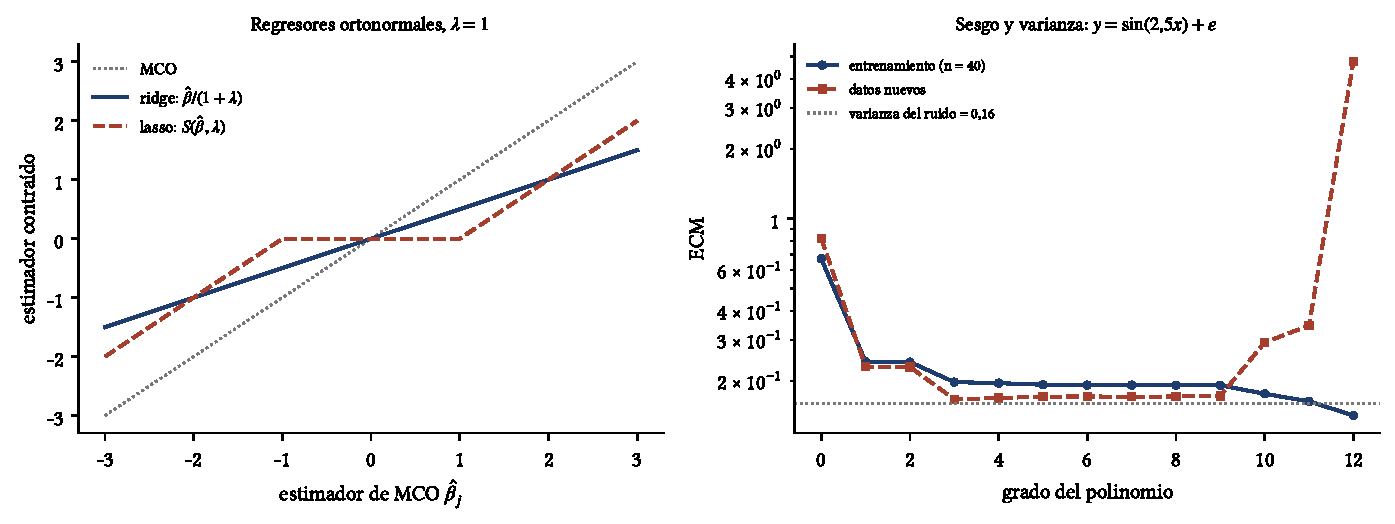
\includegraphics[width=\linewidth]{graficos/cap20_fig_teoria.pdf}
\caption{Izquierda: ridge contrae en proporción y lasso aplica un umbral suave que anula los coeficientes pequeños. Derecha: error de
entrenamiento y de datos nuevos de polinomios de grado creciente ajustados a 40 observaciones (escala logarítmica).}
\label{fig:teoria20}
\end{figure}

% ---------------------------------------------------------------------
\section{Evaluar pronósticos de rendimientos}
% ---------------------------------------------------------------------

El pronóstico de referencia es la media histórica $\bar y_t$, que no usa predictores. Campbell y Thompson (2008) definen
\[
  R^2_{OS}=1-\frac{\sum_t(y_{t+1}-\hat y_{t+1})^2}{\sum_t(y_{t+1}-\bar y_t)^2},
\]
que es positivo solo si el modelo tiene menor error cuadrático que la media. Para contrastar $H_0$: $R^2_{OS}\le0$ con modelos
anidados se usa el estadístico de Clark y West (2007), que corrige el ruido que introduce estimar parámetros que en la
población son cero: la $t$ de la media de $f_{t+1}=(y-\bar y)^2-[(y-\hat y)^2-(\bar y-\hat y)^2]$, con valor crítico unilateral.

Un $R^2$ pequeño puede valer mucho.

\begin{proposicion}[Valor de un $R^2$ pequeño]\label{prop:ct}
Sea $r_{t+1}=\mu+x_t+\varepsilon_{t+1}$, con $\E[x_t]=0$, $\Var(x_t)=R^2\sigma^2$ y $\Var(\varepsilon)=(1-R^2)\sigma^2$, y sea $S=\mu/\sigma$ la razón de
Sharpe incondicional. Un inversionista media-varianza con aversión $\gamma$ que invierte $w_t=(\mu+x_t)/[\gamma(1-R^2)\sigma^2]$ obtiene un
exceso de rendimiento esperado $\frac{S^2+R^2}{\gamma(1-R^2)}$, frente a $\frac{S^2}{\gamma}$ si ignora el predictor.
\end{proposicion}

\begin{proof}
El rendimiento esperado de la cartera condicionada en $x_t$ es $w_t(\mu+x_t)$:
\begin{align*}
  \E[w_t(\mu+x_t)] &= \frac{\E[(\mu+x_t)^2]}{\gamma(1-R^2)\sigma^2}\\
                   &= \frac{\mu^2+R^2\sigma^2}{\gamma(1-R^2)\sigma^2}\\
                   &= \frac{S^2+R^2}{\gamma(1-R^2)} .
\end{align*}
Sin el predictor, la varianza relevante es $\sigma^2$ y el peso constante $\mu/(\gamma\sigma^2)$, con rendimiento esperado
$\mu^2/(\gamma\sigma^2)=S^2/\gamma$.
\end{proof}

Con la razón de Sharpe mensual del mercado en nuestra muestra, $S=0{,}121$ y $S^2=0{,}0146$, un $R^2$ mensual de apenas 0,5\,\% aumenta el
rendimiento esperado del inversionista en
\begin{align*}
  \frac{(0{,}0146+0{,}005)/(1-0{,}005)}{0{,}0146}-1 &= \frac{0{,}0197}{0{,}0146}-1\\
                                                    &= 0{,}35,
\end{align*}
un 35\,\%. Por eso en finanzas un $R^2_{OS}$ de medio punto porcentual es económicamente relevante.

% ---------------------------------------------------------------------
\section{Clasificación: regresión logística}
% ---------------------------------------------------------------------

Para una variable binaria $y_i\in\{0,1\}$ (recesión o no, impago o no), el modelo logit es
$\Pr(y_i=1\mid\mathbf x_i)=p_i=1/(1+e^{-\mathbf x_i'\boldsymbol\beta})$.

\begin{proposicion}[Gradiente y hessiano del logit]\label{prop:logit}
La log-verosimilitud $\ell(\boldsymbol\beta)=\sum_i[y_i\ln p_i+(1-y_i)\ln(1-p_i)]$ tiene gradiente $X'(\mathbf y-\mathbf p)$ y hessiano
$-X'WX$, con $W=\operatorname{diag}(p_i(1-p_i))$. Por tanto es cóncava y el método de Newton
$\boldsymbol\beta\leftarrow\boldsymbol\beta+(X'WX)^{-1}X'(\mathbf y-\mathbf p)$ converge a su máximo único cuando existe.
\end{proposicion}

\begin{proof}
Con $\eta_i=\mathbf x_i'\boldsymbol\beta$, $\ln p_i=-\ln(1+e^{-\eta_i})$ y $\ln(1-p_i)=-\eta_i-\ln(1+e^{-\eta_i})$:
\begin{align*}
  \ell &= \sum_i\bigl[y_i\ln p_i+(1-y_i)\ln(1-p_i)\bigr]\\
       &= \sum_i\bigl[-y_i\ln(1+e^{-\eta_i})-(1-y_i)\eta_i-(1-y_i)\ln(1+e^{-\eta_i})\bigr]\\
       &= \sum_i\bigl[(y_i-1)\eta_i-\ln(1+e^{-\eta_i})\bigr].
\end{align*}
Como $\frac{d}{d\eta}\ln(1+e^{-\eta})=-\frac{e^{-\eta}}{1+e^{-\eta}}=-(1-p)$:
\begin{align*}
  \frac{\partial\ell}{\partial\eta_i} &= y_i-1+(1-p_i)\\
                                      &= y_i-p_i,\\
  \frac{\partial^2\ell}{\partial\eta_i^2} &= -\frac{dp_i}{d\eta_i}\\
                                          &= -p_i(1-p_i).
\end{align*}
Por la regla de la cadena con $\partial\eta_i/\partial\boldsymbol\beta=\mathbf x_i$, el gradiente es $\sum_i\mathbf x_i(y_i-p_i)$ y el hessiano
$-\sum_ip_i(1-p_i)\mathbf x_i\mathbf x_i'$, que es definido negativo si $X$ tiene rango completo.
\end{proof}

La calidad de un clasificador no depende de un umbral: el \emph{área bajo la curva ROC} (AUC) es la probabilidad de que un caso positivo
elegido al azar reciba una probabilidad mayor que un caso negativo, y se calcula con los rangos (el estadístico de Mann-Whitney). Vale
0,5 para un clasificador aleatorio y 1 para uno perfecto.

\paragraph{Árboles de regresión.} Un árbol divide el espacio de predictores en rectángulos con cortes binarios
($x_j\le u$ o $x_j>u$) elegidos uno a uno para minimizar la suma de cuadrados, y pronostica con la media de cada rectángulo
(Breiman, Friedman, Olshen y Stone, 1984). Captura no linealidades e interacciones sin especificarlas, pero cada corte se elige
mirando los datos: un árbol profundo memoriza el ruido. Los bosques aleatorios y el \emph{boosting} promedian muchos árboles para
reducir esa varianza.

% ---------------------------------------------------------------------
\section{Ejercicios resueltos}
% ---------------------------------------------------------------------

\begin{ejresuelto}{Un predictor a la vez}\label{ej:goyalwelch}
\enunciado Para cada uno de los diez predictores, estime la regresión predictiva $y_{t+1}=a+bx_t+u_{t+1}$ en toda la muestra y fuera de muestra
desde enero de 1957, con ventana creciente y reestimación mensual. Calcule el $R^2_{OS}$, su versión con la restricción de Campbell y
Thompson (pronóstico negativo sustituido por cero) y la prueba de Clark y West.

\solucion
\paso{Paso 1. Resultados} ($R^2$ en \%).
\begin{center}\small
\begin{tabular}{@{}lrrrrrr@{}}
\toprule
Predictor & $\hat b$ & $t$ & $R^2$ dentro & $R^2_{OS}$ & $R^2_{OS}$ CT & $p$ (CW) \\
\midrule
$dp$ & 0,689 & 1,41 & 0,35 & $-0{,}57$ & $-0{,}06$ & 0,052 \\
$ep$ & 0,790 & 1,93 & 0,38 & $-1{,}27$ & $-0{,}41$ & 0,218 \\
$de$ & 0,089 & 0,11 & 0,00 & $-0{,}71$ & $-0{,}69$ & 0,998 \\
CAPE & $-1{,}141$ & $-2{,}21$ & 0,73 & $-2{,}50$ & $-1{,}39$ & 0,083 \\
$lty$ & $-0{,}081$ & $-1{,}48$ & 0,18 & $-0{,}76$ & 0,19 & 0,078 \\
$tbl$ & $-0{,}094$ & $-1{,}72$ & 0,29 & $-0{,}13$ & 0,51 & 0,071 \\
$tms$ & 0,179 & 1,13 & 0,15 & $-0{,}03$ & 0,24 & 0,221 \\
Inflación & $-0{,}047$ & $-0{,}64$ & 0,12 & 0,15 & 0,15 & 0,215 \\
Momentum & 0,010 & 0,62 & 0,14 & $-0{,}25$ & $-0{,}11$ & 0,533 \\
Volatilidad & 0,067 & 0,51 & 0,11 & 0,21 & 0,21 & 0,029 \\
\bottomrule
\end{tabular}
\end{center}
Dentro de la muestra, el mejor predictor es el CAPE ($t=-2{,}21$, $R^2=0{,}73$\,\%). Fuera de muestra es el peor: $R^2_{OS}=-2{,}50$\,\%. Ocho
de los diez predictores pronostican peor que la media histórica. Es el resultado de Goyal y Welch (2008) en estos datos.

\paso{Paso 2. La restricción económica.} Sustituir los pronósticos negativos de la prima por cero, porque un inversionista racional
no espera una prima negativa, mejora todos los modelos y vuelve positivos a $lty$, $tbl$ y $tms$. La prueba de Clark y West, que
reconoce que un modelo anidado con un coeficiente verdadero pequeño puede tener $R^2_{OS}<0$ por el ruido de estimación, rechaza
al 5\,\% solo para la volatilidad ($p=0{,}029$) y queda cerca para $dp$ ($p=0{,}052$).

\paso{Paso 3. ¿Cuándo funcionan?} La Figura~\ref{fig:goyalwelch} acumula la diferencia de errores cuadráticos: sube cuando el modelo
gana. La razón dividendo/precio acumula ventaja hasta 1990 y la pierde por completo entre 1995 y 2000; el CAPE pierde desde el
principio y sobre todo en esa burbuja, cuando las valuaciones altas anunciaban caídas que tardaron años en llegar.

\codigoweb{cap20_ej01}
\salidaR{cap20_ej01_R.txt}
\lectura{cap20_ej01}

\RvsPy El archivo de predictores se construye una sola vez en Python y ambos lenguajes lo leen. En el pronóstico del mes $i$, la
muestra de entrenamiento son los pares $(x_s,y_{s+1})$ con $y_{s+1}$ ya observado: en R, las filas \texttt{1:(i - 1)}; en Python,
\texttt{[:i]}. Un error de una posición en este índice es la forma más común de introducir información del futuro, y en una primera
versión de este código Python usaba una observación menos que R: la comparación entre ambos lenguajes lo detectó.

\begin{figure}[ht]
\centering
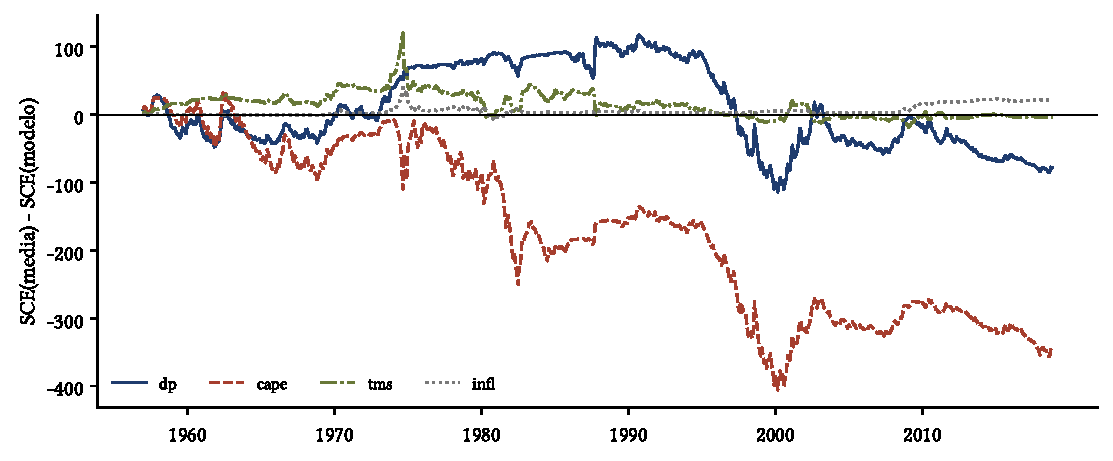
\includegraphics[width=\linewidth]{graficos/cap20_ej01_goyal_welch.pdf}
\caption{Diferencia acumulada entre el error cuadrático de la media histórica y el de cada modelo univariado. Una curva creciente
indica que el modelo gana.}
\label{fig:goyalwelch}
\end{figure}

\begin{conclusion}
La significancia dentro de la muestra no garantiza capacidad predictiva fuera de ella. Los predictores clásicos de la prima de mercado
pronostican, en el mejor de los casos, apenas mejor que la media.
\end{conclusion}
\end{ejresuelto}

\begin{ejresuelto}{Todos los predictores con contracción}\label{ej:contraccion}
\enunciado Use todos los predictores a la vez con MCO, ridge, red elástica ($\alpha=0{,}5$) y lasso, reestimando cada enero desde 1957. Elija
$\lambda$ en una malla de 30 valores con los últimos 120 meses de cada muestra de entrenamiento.

\solucion
\paso{Paso 1. Colinealidad exacta.} $de=dp-ep$ y $tms=lty-tbl$ son combinaciones lineales exactas de otros predictores: con los diez,
$X'X$ es singular y MCO no tiene solución única. R lo detecta (``system is computationally singular''); Python, por redondeo, devolvía
un resultado sin advertir. Usamos ocho predictores.

\paso{Paso 2. Resultados.}
\begin{center}\small
\begin{tabular}{@{}lrrrr@{}}
\toprule
Modelo & $R^2_{OS}$ (\%) & $R^2_{OS}$ CT (\%) & $p$ (CW) & $\lambda$ mediano \\
\midrule
MCO (8 predictores) & $-6{,}04$ & $-2{,}93$ & 0,531 & -- \\
Ridge & $-1{,}12$ & 0,17 & 0,370 & 3,324 \\
Red elástica & $-2{,}33$ & $-0{,}94$ & 0,692 & 0,846 \\
Lasso & $-1{,}95$ & $-0{,}90$ & 0,605 & 0,499 \\
\bottomrule
\end{tabular}
\end{center}
MCO con todos los predictores es desastroso: $R^2_{OS}=-6{,}04$\,\%. Sus pronósticos tienen una desviación estándar de 1,01\,\% mensual, doce
veces la de la media histórica (0,08\,\%): reacciona con fuerza a variaciones de los predictores que solo son ruido. La contracción
reduce esa volatilidad (0,44 con ridge, 0,52 con lasso) y el error, pero no lo suficiente para superar a la media.

\paso{Paso 3. Qué selecciona el lasso.} En promedio, 2,56 predictores; en 14 de las 62 reestimaciones, ninguno (el pronóstico es la
media). El CAPE entra en el 77\,\% de las reestimaciones, el momentum en el 42\,\% y la volatilidad apenas en el 6\,\% (Figura~\ref{fig:contraccion}).

\codigoweb{cap20_ej02}
\salidaR{cap20_ej02_R.txt}
\lectura{cap20_ej02}

\RvsPy El descenso por coordenadas está programado igual en ambos lenguajes, con la misma tolerancia y arranque en caliente a lo largo
de la malla de $\lambda$ (cada ajuste parte de la solución del $\lambda$ anterior). Los predictores se estandarizan con la media y la
desviación estándar de la muestra de entrenamiento (dividiendo entre $n$), nunca con la de toda la muestra. Los paquetes de referencia son
\texttt{glmnet} en R y \texttt{sklearn.linear\_model.ElasticNet} en Python, que parametrizan la penalización de la misma forma; el bucle en
Python tarda unos dos minutos, frente a 30 segundos en R.

\begin{figure}[ht]
\centering
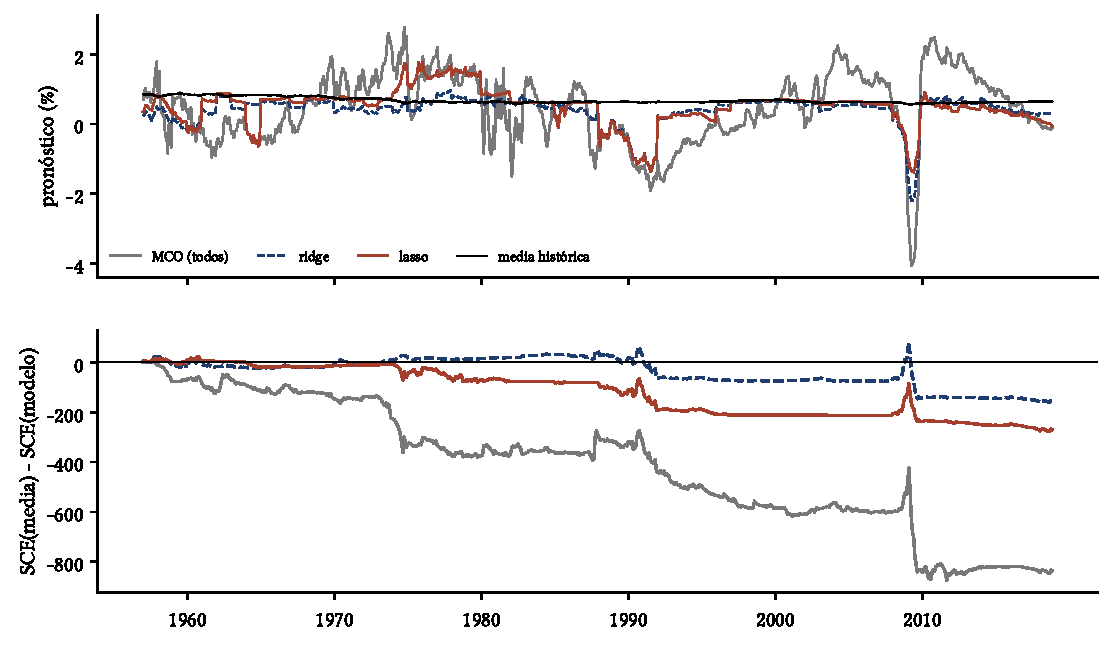
\includegraphics[width=\linewidth]{graficos/cap20_ej02_contraccion.pdf}
\caption{Arriba: pronósticos mensuales de MCO, ridge, lasso y la media histórica. Abajo: diferencia acumulada de errores cuadráticos
frente a la media.}
\label{fig:contraccion}
\end{figure}

\begin{conclusion}
Con una señal tan débil, más variables empeoran el pronóstico, y la contracción solo atenúa el daño. La validación temporal elige
penalizaciones altas, es decir, pronósticos cercanos a la media: los datos le dicen al algoritmo que confíe poco en los predictores.
\end{conclusion}
\end{ejresuelto}

\begin{ejresuelto}{Combinación de pronósticos y su valor económico}\label{ej:combinacion}
\enunciado Combine los diez pronósticos univariados del Ejercicio~\ref{ej:goyalwelch} con su media y su mediana (Rapach, Strauss y Zhou, 2010) y
compare con regresiones sobre 1, 2 y 3 componentes principales. Evalúe el valor económico para un inversionista media-varianza con aversión 3.

\solucion
\paso{Paso 1. Precisión.}
\begin{center}\small
\begin{tabular}{@{}lrrr@{}}
\toprule
Modelo & $R^2_{OS}$ (\%) & CW & $p$ \\
\midrule
Combinación (media) & 0,61 & 2,13 & 0,017 \\
Combinación (mediana) & 0,50 & 2,29 & 0,011 \\
Componentes principales ($k=1$) & $-0{,}36$ & 2,16 & 0,016 \\
Componentes principales ($k=2$) & $-0{,}78$ & 2,19 & 0,014 \\
Componentes principales ($k=3$) & $-1{,}53$ & 2,04 & 0,021 \\
\bottomrule
\end{tabular}
\end{center}
La media simple de los diez pronósticos, ninguno de los cuales supera claramente a la media histórica, tiene $R^2_{OS}=0{,}61$\,\% y
supera a la media con $p=0{,}017$. La combinación es una forma extrema de contracción: cada predictor recibe un peso fijo de 1/10, sin
estimar, y los errores de los distintos modelos se compensan. Su desviación estándar es 0,11\,\%, apenas mayor que la de la media
histórica (Figura~\ref{fig:combinacion}).

\paso{Paso 2. Valor económico.} El inversionista invierte en acciones $w_t=\hat y_{t+1}/(\gamma\hat\sigma^2_t)$, con $\gamma=3$, la varianza de los
últimos 60 meses y el peso acotado entre 0 y 150\,\%. Su equivalente cierto anual es
\begin{align*}
  EC &= 12\Bigl[\bar r_p-\tfrac{\gamma}{2}\hat\sigma^2_p\Bigr],\\
  EC_{\text{combinación}}-EC_{\text{media}} &= 7{,}570-6{,}617\\
                                            &= 0{,}953\ \text{puntos porcentuales por año}.
\end{align*}
Casi un punto anual: el inversionista pagaría hasta 0,95\,\% de su patrimonio cada año por usar la combinación. Con solo $dp$, en cambio,
pierde 0,88 puntos.

\codigoweb{cap20_ej03}
\salidaR{cap20_ej03_R.txt}
\lectura{cap20_ej03}

\RvsPy Con rendimientos en porcentaje, el peso óptimo es $100\,\hat y/(\gamma\hat\sigma^2)$ y la penalización por varianza se divide entre 100; una
primera versión del código olvidó esas escalas y daba equivalentes ciertos absurdos de más de 400\,\% anual. Los autovectores de
\texttt{eigen} (R) y \texttt{np.linalg.eigh} (Python) pueden tener signos opuestos, pero eso no cambia la regresión sobre los componentes.

\begin{figure}[ht]
\centering
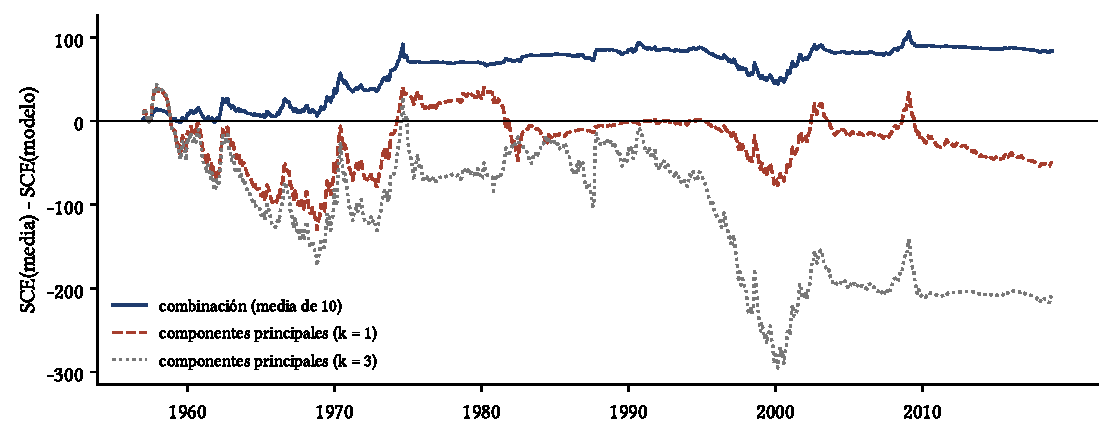
\includegraphics[width=\linewidth]{graficos/cap20_ej03_combinacion.pdf}
\caption{Diferencia acumulada de errores cuadráticos frente a la media histórica de la combinación y de las regresiones sobre componentes
principales.}
\label{fig:combinacion}
\end{figure}

\begin{conclusion}
El mejor ``modelo'' no es el más sofisticado sino el más humilde: promediar pronósticos simples. Y un $R^2_{OS}$ de 0,6\,\% vale casi un punto
porcentual anual para un inversionista, como anticipa la Proposición~\ref{prop:ct}.
\end{conclusion}
\end{ejresuelto}

\begin{ejresuelto}{¿Anuncia la curva las recesiones?}\label{ej:recesiones20}
\enunciado Con los datos de 1946 a 1991, estime un logit de la probabilidad de que el mes $t+h$ esté en recesión según la pendiente de la curva
$y_{120}-y_3$ en $t$, para $h=3$, 6, 12, 18 y 24 meses. Para $h=12$, calcule la tabla de clasificación con dos umbrales y la AUC fuera de
muestra desde 1965.

\solucion
\paso{Paso 1. Horizontes.}
\begin{center}\small
\begin{tabular}{@{}rrrrr@{}}
\toprule
$h$ & $\hat\beta_1$ & ee & Pseudo $R^2$ & AUC \\
\midrule
3 & $-0{,}576$ & 0,108 & 0,063 & 0,660 \\
6 & $-0{,}930$ & 0,127 & 0,141 & 0,752 \\
12 & $-1{,}174$ & 0,145 & 0,199 & 0,819 \\
18 & $-0{,}718$ & 0,114 & 0,095 & 0,715 \\
24 & $-0{,}237$ & 0,100 & 0,011 & 0,557 \\
\bottomrule
\end{tabular}
\end{center}
La pendiente predice mejor a un año: es el resultado de Estrella y Mishkin (1998). Agregar el nivel de la tasa corta no ayuda ($LR=0{,}17$).

\paso{Paso 2. Probabilidades.} Con $\hat\beta_0=-0{,}695$ y $\hat\beta_1=-1{,}174$:
\begin{align*}
  \Pr(\text{recesión}\mid\text{pendiente}=0) &= \frac{1}{1+e^{0{,}695}}\\
                                            &= 0{,}333,\\
  \Pr(\text{recesión}\mid\text{pendiente}=2) &= \frac{1}{1+e^{0{,}695+2\times1{,}174}}\\
                                            &= \frac{1}{1+e^{3{,}043}}\\
                                            &= 0{,}046 .
\end{align*}
La probabilidad supera el 50\,\% solo cuando la curva está invertida en más de 0,59 puntos.

\paso{Paso 3. Umbrales.} Con umbral 0,5, el modelo detecta solo 23 de 95 meses de recesión (sensibilidad 0,24) con pocas falsas alarmas
(especificidad 0,97). Con umbral igual a la frecuencia muestral (0,183), detecta 71 (sensibilidad 0,75) a costa de 112 falsas alarmas
(especificidad 0,74). La AUC resume todos los umbrales: 0,819 dentro de la muestra y 0,835 fuera de muestra desde 1965, usando solo
recesiones ya observadas en cada fecha (Figura~\ref{fig:recesiones20}).

\codigoweb{cap20_ej04}
\salidaR{cap20_ej04_R.txt}
\lectura{cap20_ej04}

\RvsPy Newton-Raphson está programado en ambos lenguajes; \texttt{glm(..., family = binomial)} en R y \texttt{statsmodels.Logit} en Python dan los
mismos coeficientes. La AUC usa los rangos promedio, de modo que los empates cuentan un medio. En el ejercicio fuera de muestra se supone
que el estado de la economía se conoce de inmediato; en la práctica el NBER fecha las recesiones con meses o años de retraso, lo que hace la
evaluación algo optimista.

\begin{figure}[ht]
\centering
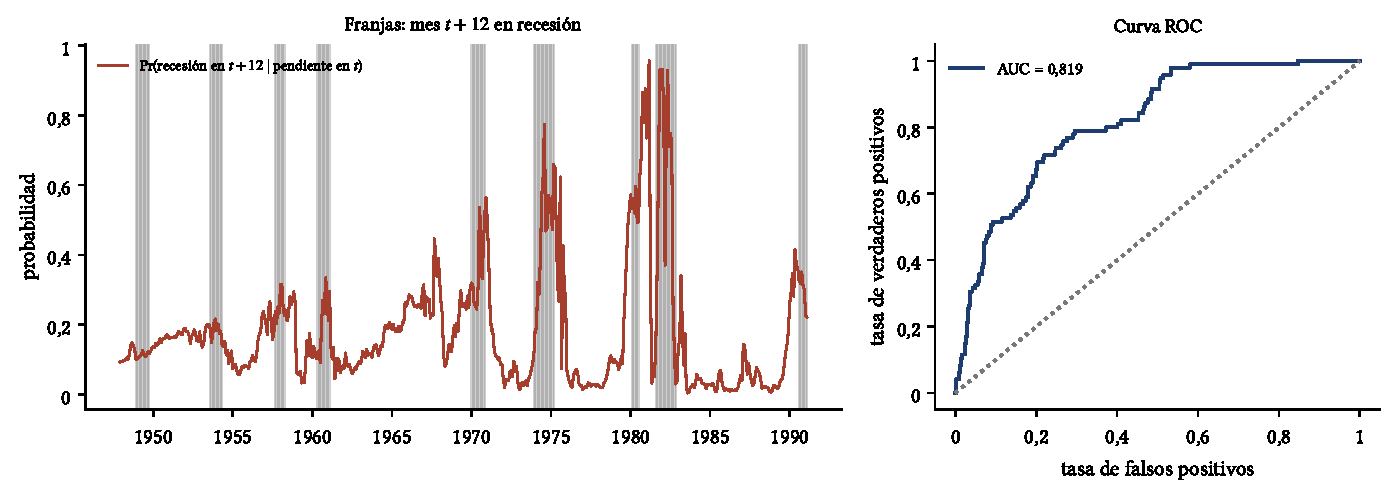
\includegraphics[width=\linewidth]{graficos/cap20_ej04_recesiones.pdf}
\caption{Izquierda: probabilidad estimada de recesión 12 meses después, con las franjas grises en los meses $t+12$ que estuvieron en recesión.
Derecha: curva ROC dentro de la muestra.}
\label{fig:recesiones20}
\end{figure}

\begin{conclusion}
Una sola variable financiera, la pendiente de la curva, clasifica bien las recesiones de un año después. El umbral de decisión depende del
costo relativo de una falsa alarma y de una recesión no anticipada, y la AUC permite comparar modelos sin elegirlo.
\end{conclusion}
\end{ejresuelto}

\begin{ejresuelto}{Árboles y sobreajuste}\label{ej:arboles}
\enunciado Entrene árboles de regresión de profundidad 0 a 6 (hojas de al menos 24 meses) con los ocho predictores de 1927 a 1980, y evalúelos en
1981--2018. Compare con MCO.

\solucion
\paso{Paso 1. Entrenamiento frente a prueba.}
\begin{center}\small
\begin{tabular}{@{}rrrrr@{}}
\toprule
Profundidad & Hojas & ECM entrenamiento & ECM prueba & $R^2$ prueba (\%) \\
\midrule
0 & 1 & 35,56 & 18,83 & 0,00 \\
1 & 2 & 34,01 & 20,83 & $-10{,}59$ \\
2 & 3 & 33,02 & 20,77 & $-10{,}29$ \\
4 & 6 & 31,99 & 20,94 & $-11{,}22$ \\
6 & 10 & 31,05 & 23,11 & $-22{,}70$ \\
\bottomrule
\end{tabular}
\end{center}
Cada corte reduce el error de entrenamiento y aumenta el de prueba. El mejor árbol es el que no corta nada, es decir, la media
(Figura~\ref{fig:arboles}). MCO lineal con los ocho predictores también pierde frente a la media: $R^2=-7{,}79$\,\%.

\paso{Paso 2. Qué aprende el árbol.} El de profundidad 2 separa 24 meses con CAPE muy bajo ($\ln\text{CAPE}\le2{,}18$, un CAPE menor que 8,8),
con un exceso de rendimiento medio de 6,95\,\% mensual, y 28 meses con deflación fuerte (inflación rezagada menor que $-3{,}44$\,\%), con
$-4{,}26$\,\%. Los primeros son meses de 1932--1933, 1942, 1974 y 1979--1980; los segundos, de 1930--1933 y 1938. Con 640 meses, el árbol
aísla unos pocos episodios extraordinarios, sobre todo de la Gran Depresión, que no se repitieron después de 1980.

\codigoweb{cap20_ej05}
\salidaR{cap20_ej05_R.txt}
\lectura{cap20_ej05}

\RvsPy El árbol se construye recursivamente en ambos lenguajes con una búsqueda exhaustiva de cortes en los puntos medios entre valores
consecutivos; los ordenamientos estables (\texttt{order(..., method = "radix")} y \texttt{np.argsort(..., kind = "stable")}) garantizan los mismos
desempates. Los paquetes de referencia (\texttt{rpart}, \texttt{sklearn.tree}) agregan poda por complejidad y validación cruzada, que aquí haría
lo mismo que la tabla: elegir la profundidad cero.

\begin{figure}[ht]
\centering
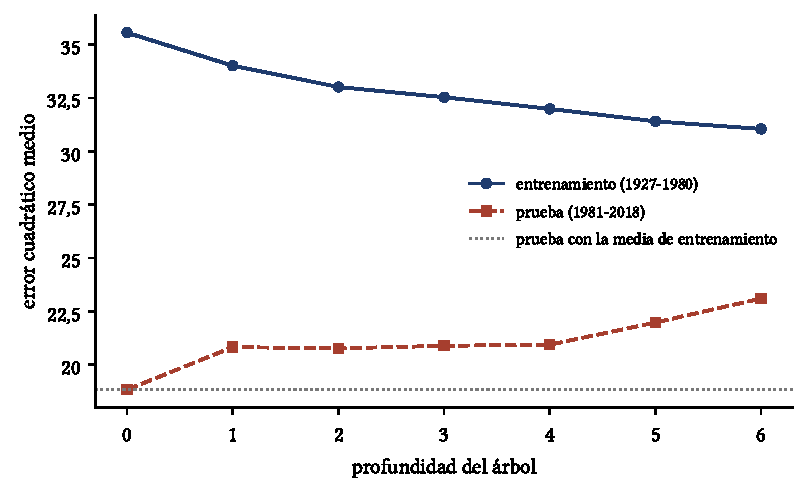
\includegraphics[width=0.78\linewidth]{graficos/cap20_ej05_arboles.pdf}
\caption{Error cuadrático medio de árboles de profundidad creciente en el período de entrenamiento y en el de prueba.}
\label{fig:arboles}
\end{figure}

\begin{conclusion}
Los métodos flexibles necesitan muchos datos y una señal estable. Con la prima de mercado agregada no hay ninguna de las dos cosas, y un árbol
solo memoriza la historia. En el corte transversal de miles de acciones, con millones de observaciones, los mismos métodos sí encuentran
estructura (Gu, Kelly y Xiu, 2020).
\end{conclusion}
\end{ejresuelto}

% ---------------------------------------------------------------------
\section{Ejercicios propuestos}
% ---------------------------------------------------------------------

\begin{enumerate}[label=\textbf{\thechapter.\arabic*},leftmargin=*,itemsep=6pt]
  \item Con regresores ortonormales, $\hat\beta=(2{,}0;\,0{,}5;\,-1{,}2)$ y $\lambda=0{,}8$, calcule ridge y lasso. \textit{Respuesta: ridge
  $(1{,}111;\,0{,}278;\,-0{,}667)$; lasso $(1{,}2;\,0;\,-0{,}4)$.}

  \item Con $S=0{,}12$ mensual y $R^2=1$\,\%, ¿en qué proporción aumenta el rendimiento esperado del inversionista de la Proposición~\ref{prop:ct}?
  \textit{Respuesta: $(0{,}0144+0{,}01)/0{,}99/0{,}0144-1=0{,}71$, un 71\,\%.}

  \item Un logit tiene $\beta_0=-0{,}7$ y $\beta_1=-1{,}2$. Calcule la probabilidad con $x=-1$ y el efecto marginal en ese punto.
  \textit{Respuesta: $p=1/(1+e^{-0{,}5})=0{,}622$; $\beta_1p(1-p)=-0{,}282$.}

  \item Demuestre que la AUC calculada con rangos es igual a la proporción de pares (positivo, negativo) en que el positivo tiene mayor puntaje.

  \item Demuestre que con $X'X/n=I$ la red elástica es $S(\hat\beta_j,\lambda\alpha)/(1+\lambda(1-\alpha))$.

  \item \emph{(Simulación.)} Genere 1\,000 meses de $y_{t+1}=0{,}1x_t+\varepsilon_{t+1}$ con $x$ AR(1) de persistencia 0,98 y $R^2=0{,}5$\,\%, y 20 predictores
  irrelevantes. Compare el $R^2_{OS}$ de MCO, lasso y la combinación.

  \item \emph{(Con datos del BCRP.)} Prediga la dirección del tipo de cambio sol-dólar del mes siguiente con un logit y diferenciales de tasas,
  y evalúe la AUC fuera de muestra.

  \item \emph{(Con datos.)} Repita el Ejercicio~\ref{ej:goyalwelch} empezando la evaluación en 1990. ¿Cambia el ranking de predictores?
\end{enumerate}

% ---------------------------------------------------------------------
\section{Resumen de fórmulas}
% ---------------------------------------------------------------------

\begin{table}[H]
\centering\small
\begin{tabular}{@{}ll@{}}
\toprule
Concepto & Fórmula \\
\midrule
Sesgo y varianza & $\E[(y_0-\hat f)^2]=\sigma^2+\text{sesgo}^2+\Var(\hat f)$ \\
Red elástica & $\frac1{2n}\lVert\mathbf y-X\boldsymbol\beta\rVert^2+\lambda[\alpha\lVert\boldsymbol\beta\rVert_1+\frac{1-\alpha}{2}\lVert\boldsymbol\beta\rVert_2^2]$ \\
Ortonormal & ridge $\hat\beta/(1+\lambda)$;\quad lasso $\operatorname{signo}(\hat\beta)\max(|\hat\beta|-\lambda,0)$ \\
Descenso por coordenadas & $\beta_j\leftarrow S(\mathbf x_j'\mathbf r_{-j}/n,\lambda\alpha)/(1+\lambda(1-\alpha))$ \\
$R^2$ fuera de muestra & $1-\sum(y-\hat y)^2/\sum(y-\bar y)^2$ \\
Clark y West & $f=(y-\bar y)^2-[(y-\hat y)^2-(\bar y-\hat y)^2]$;\quad $t$ de $\bar f$ \\
Valor de un $R^2$ & $\frac{S^2+R^2}{\gamma(1-R^2)}$ frente a $\frac{S^2}{\gamma}$ \\
Logit & $p=1/(1+e^{-\mathbf x'\boldsymbol\beta})$;\quad $\nabla\ell=X'(\mathbf y-\mathbf p)$;\quad $\nabla^2\ell=-X'WX$ \\
AUC & $\Pr(\text{puntaje de un positivo}>\text{puntaje de un negativo})$ \\
\bottomrule
\end{tabular}
\caption{Fórmulas principales del Capítulo 20.}
\end{table}

\section*{Referencias}
\begin{itemize}[leftmargin=*]
  \item Breiman, L., Friedman, J., Olshen, R. y Stone, C. (1984). \emph{Classification and Regression Trees}. Wadsworth.
  \item Campbell, J. Y. y Thompson, S. B. (2008). Predicting excess stock returns out of sample: Can anything beat the historical average?
        \emph{Review of Financial Studies}, 21(4), 1509--1531.
  \item Clark, T. E. y West, K. D. (2007). Approximately normal tests for equal predictive accuracy in nested models. \emph{Journal of
        Econometrics}, 138(1), 291--311.
  \item Estrella, A. y Mishkin, F. S. (1998). Predicting U.S. recessions: Financial variables as leading indicators. \emph{Review of
        Economics and Statistics}, 80(1), 45--61.
  \item Friedman, J., Hastie, T. y Tibshirani, R. (2010). Regularization paths for generalized linear models via coordinate descent.
        \emph{Journal of Statistical Software}, 33(1), 1--22.
  \item Goyal, A. y Welch, I. (2008). A comprehensive look at the empirical performance of equity premium prediction. \emph{Review of
        Financial Studies}, 21(4), 1455--1508.
  \item Gu, S., Kelly, B. y Xiu, D. (2020). Empirical asset pricing via machine learning. \emph{Review of Financial Studies}, 33(5),
        2223--2273.
  \item Hastie, T., Tibshirani, R. y Friedman, J. (2009). \emph{The Elements of Statistical Learning}, 2.ª ed. Springer.
  \item Hoerl, A. E. y Kennard, R. W. (1970). Ridge regression: Biased estimation for nonorthogonal problems. \emph{Technometrics}, 12(1),
        55--67.
  \item Rapach, D. E., Strauss, J. K. y Zhou, G. (2010). Out-of-sample equity premium prediction: Combination forecasts and links to the real
        economy. \emph{Review of Financial Studies}, 23(2), 821--862.
  \item Tibshirani, R. (1996). Regression shrinkage and selection via the lasso. \emph{Journal of the Royal Statistical Society, Series B},
        58(1), 267--288.
  \item Zou, H. y Hastie, T. (2005). Regularization and variable selection via the elastic net. \emph{Journal of the Royal Statistical
        Society, Series B}, 67(2), 301--320.
\end{itemize}
